\lfoot{Autor: Raphael Simsek}
\subsection{Analyse und Verbesserung des Fahrstils}

\todo{Bezug auf wie sie in der Graphik unten erkennen können, auf wie sie in Abb. 1 erkennen können ändern, Kapitel Referenzen genauso durch gehen}
Aus persönlicher Erfahrung geht hervor, dass es bei der Ausbildung zum Fahrer eines Kraftfahrzeugs einigen Verbesserungsbedarf gibt. Häufig kann nicht immer der Fahrlehrer einem Fahrschüler einen nachhaltigen oder wünschenswerten Fahrstil näher bringen. Dies ist nämlich oft ein zeitintensiver Prozess ist. Aus diesem Grund wurden Methoden gesammelt und entwickelt, welche die Problematik aufholen sollen.

\subsubsection{Sozialer Zwang}
Immer mehr Appplikationen implementierne eine Anbindung zu sozialen Medien wie Facebook, Twitter und Reddit. Mittels dieser Abindung wird die Möglichkeit geboten, die Information, welche von der Applikation bezogen worde, auf den soziallen Plattformen zu posten und zu \textit{sharen}. \cite{SIMR.CH1-fahrstil-analyse.GewohnheitenLoslassen}. Eines der bekanntesten österreichischen Beispiele ist das App-System von Runtastic \cite{SIMR.CH1-Fahrstil-Analyse.BusinessplanRuntastic}.
Nur im Bezug auf das Autofahren konnte kein derartiges System  gefunden werden.

Zu Beginn des Diplomprojektes gab es folglich keine Möglichkeiten für verbesserungswillige Autofahrer ihren Fahrstil zu verbessern und dies dann sogar zu teilen. 

\paragraph{Peer-Pressure} 
\begin{wrapfigure}{r}{0.6\textwidth}\centering
    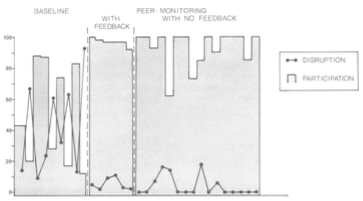
\includegraphics[width=0.6\textwidth]{images/peerPressure}
    \caption{Verhaltensanalyse von Kindern bei gegenseitigem Monitoring \cite{SIMR.CH1-fahrstil-analyse.PeerPressure}} \label{Fig:imgPeerPressure}
\end{wrapfigure}
Das Teilen der Fahrstilanalyse trägt durch \textit{Peer-Pressure}  dazu bei, dass die Nutzer andere Nutzer überbieten möchten und so ihren eigenen Fahrstil verbessern. Diese Theorie bestätigt eine Studie, bei der sich Schüler gegenseitig beobachten. Die Studie zeigt, dass von gleichgesinnten umgebene und überwachte Schüler (hier Social Network) sich selbst angepasster verhalten und sich auf Ihre Vernunft besinnen \cite{SIMR.CH1-fahrstil-analyse.PeerPressure}. Es würden sich Fahrer folglich genauso vernünftiger fahren, wie sich die Schüler in dieser Studie verhalten haben.

Bei der Evaluierung des Project Scope fiel uns besonders auf, dass eine Analyse-Funktion für die nachhaltige Verbesserung des Fahrstils behilflich sein könnte. Es wurde für diese Analyse evaluiert, welche Funktionalitäten am Wichtigsten sind, wobei diese auch innerhalb der Diplomarbeit realisierbar sein sollten.

\subsubsection{Fahrkomfortanalyse}
Eine Analyse der Wirkung von Beschleunigungskräften auf den Fahrer, ist üblicherweise nur bei Sportwagen verbaut. Bei derartigen Fahrzeugen wird die Funktionalität nicht für das frühzeitige Verbessern des Fahrstils eines Fahrers verwendet, sondern für die Optimierung von Rundenzeiten auf einer Rennstrecke.

\begin{figure}[!htb]\centering
	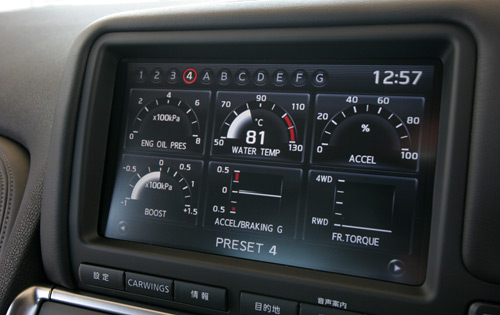
\includegraphics[width=0.6\textwidth]{images/gtrMultifunc}
	\caption{Analyse Möglichkeiten bei einem Nissan GT-R (R35) \cite{SIMR.CH1-Fahrstil-Analyse.GTRMultifunc}}\label{Fig:imgGTR}
\end{figure}

Im Kontrast zu bisher etablierten Möglichkeiten ist die Anzeige der Fahrgastbequemlichkeit anhand fundamental anderen Parametern aufgebaut. Sie soll dem Fahrer aufzeigen welche Kurven dieser zu schnell durchfahren hat. Als Maß für die Bequemlichkeit wird dabei die Beschleunigungskraft in g [Kraft/Masse] herangezogen. Genauere Ausführungen zu diesem Thema, können unter Kapitel \ref{subsec:fahrgastkomfortanalyse} gefunden werden.

\subsubsection{Schaltvorschlag}
Der bisherige Schaltvorschlag in einem kostengünstigen, gebrauchten Auto ist oft äußerst simpel gehalten. Es wird hierbei ab einer gewissen Drehzahl der darauffolgende Gang vorgeschlagen oder nur auf den Normzyklus optimiert \cite{SIMR.CH1-Fahrstil-Analyse.Schaltempfehlung}.
\paragraph{Normzyklus}
Der Normzyklus ist insbesondere aufgrund des VW-Skandals bekannt geworden. Es erkennt die Motorsteuerung nämlich, wenn ein Abgastest gefahren wird. Dieser wird in der Fachsprache als Normzyklus bezeichnet wird \cite{SIMR.CH1-fahrstil-analyse.Normzyklus}. Der \textit{modifizierte neue europäische Fahrzyklus (MNEFZ)} ist der Normzyklus, der innerhalb der EU verwendet wird um den Normverbrauch eines Fahrzeuges zu errechnen. Dieser umfasst insgesamt 1180 Sekunden, wovon 780 Sekunden unter Stadtbedingungen und 400 Sekunden über Land gefahren werden. Der MNEFZ wird häufig wegen spritsparender Maßnahmen, vor dem Test, kritisiert. Diese Tricks dürfen von den Autoherstellern eingesetzt werden und umfassen die Erhöhung des Reifendrucks oder das Abklemmen der Lichtmaschine. Ferner wird der Test ohne eingeschalteter Klimaanlage oder anderer \textit{Creature-Comforts} gefahren. Herstellerangaben werden in Europa nämlich selten hinterfragt \cite{SIMR.CH1-fahrstil-analyse.MNEFZ}. In den USA mussten, im Gegensatz dazu, Automobilhersteller bereits in vielen Fällen hohe Entschädigungen zahlen für falsche Verbrauchsangaben bezahlen \cite{SIMR.CH1-fahrstil-analyse.falscherVerbrauchUS}.
\paragraph{Carnot-Prozess}
\todo{sanfter Einführen, wofür brauchen wir den Carnot Prozess}
In diesem musste in Erfahrung gebracht werden, wie ein Motor funktioniert und welche Faktoren diesen beeinflussen. Vor allem ist dabei der Motorwirkungsgrad herausgestochen, welcher mit dem Carnot Prozess definiert ist. Dieser bestimmt wie viel Energie der Motor pro eingespritztem Kraftstoff definiert und ist damit bestimmt damit die Leistung die ein Motor emitiert. Ursprünglich war der Carnot Prozess definiert um einen Kreisprozess zu erläutern und wurde konnte folglich auch auf Motoren angewandt werden.
Der Motorwirkungsgrad nach dem Carnot-Prozess, wird für bekannte Schaltvorschläge in Serienfahrzeugen meist noch nicht verwendet. Der Carnot-Prozess beschreibt die Errechnung des \textit{theoretisch möglichen} Motorwirkungsgrad, ohne dem Hinzuziehen von natürlichen Einflussgrößen. Diese können u.a. Reibung, Temperatur und Dichte sein \cite{SIMR.CH1-Fahrstil-Analyse.CarnotWirkungsgrad}. Genauere Ausführungen zu diesem Thema können im Kaptiel \ref{subsec:motorwirkungsgrad} gefunden werden. 

\subsubsection{Schadstoffausstoß}
Eine Live-Messung von \ce{CO2} Werten während der Fahrt ist zumeist eine Schätzung, welche durch den Bordcomputer durchgeführt wird und noch bei wenigen Modellen Einsatz findet. Grenzwerte oder gar eine Analysefunktionalität gibt es in dieser Hinsicht aber nicht. Die \ce{CO2} Werte werden in Zukunft allerdings noch weitaus relevanter. Denn, wie im folgenden Kapitel \ref{subsec:umweltbelastungco2} ausführlich beschrieben, wird bis 2020 versucht wird einen Durschnittsaustoß von 95 g/km zu erzielen. \cite{SIMR.CH1-Fahrstil_Analyse.EUVerordCO2} Deshalb wurde die Zukunftssicherheit momentaner Bordcomputer in dieser Hinsicht bemängelt.
